\documentclass[10pt, a5paper]{article}
\usepackage{pdfpages}
\usepackage{parallel}
\usepackage[T2A]{fontenc}
\usepackage{ucs}
\usepackage[utf8x]{inputenc}
\usepackage[polish,english,russian]{babel}
\usepackage{hyperref}
\usepackage{rotating}
\usepackage[inner=2cm,top=1.8cm,outer=2cm,bottom=2.3cm,nohead]{geometry}
\usepackage{listings}
\usepackage{graphicx}
\usepackage{wrapfig}
\usepackage{longtable}
\usepackage{indentfirst}
\usepackage{array}
\newcolumntype{P}[1]{>{\raggedright\arraybackslash}p{#1}}
\frenchspacing
\usepackage{fixltx2e} %text sub- and superscripts
\usepackage{icomma} % коскі ў матэматычным рэжыме
\PreloadUnicodePage{4}

\newcommand{\longpage}{\enlargethispage{\baselineskip}}
\newcommand{\shortpage}{\enlargethispage{-\baselineskip}}

\def\switchlang#1{\expandafter\csname switchlang#1\endcsname}
\def\switchlangbe{
\let\saverefname=\refname%
\def\refname{Літаратура}%
\def\figurename{Іл.}%
}
\def\switchlangen{
\let\saverefname=\refname%
\def\refname{References}%
\def\figurename{Fig.}%
}
\def\switchlangru{
\let\saverefname=\refname%
\let\savefigurename=\figurename%
\def\refname{Литература}%
\def\figurename{Рис.}%
}

\hyphenation{admi-ni-stra-tive}
\hyphenation{ex-pe-ri-ence}
\hyphenation{fle-xi-bi-li-ty}
\hyphenation{Py-thon}
\hyphenation{ma-the-ma-ti-cal}
\hyphenation{re-ported}
\hyphenation{imp-le-menta-tions}
\hyphenation{pro-vides}
\hyphenation{en-gi-neering}
\hyphenation{com-pa-ti-bi-li-ty}
\hyphenation{im-pos-sible}
\hyphenation{desk-top}
\hyphenation{elec-tro-nic}
\hyphenation{com-pa-ny}
\hyphenation{de-ve-lop-ment}
\hyphenation{de-ve-loping}
\hyphenation{de-ve-lop}
\hyphenation{da-ta-ba-se}
\hyphenation{plat-forms}
\hyphenation{or-ga-ni-za-tion}
\hyphenation{pro-gramming}
\hyphenation{in-stru-ments}
\hyphenation{Li-nux}
\hyphenation{sour-ce}
\hyphenation{en-vi-ron-ment}
\hyphenation{Te-le-pathy}
\hyphenation{Li-nux-ov-ka}
\hyphenation{Open-BSD}
\hyphenation{Free-BSD}
\hyphenation{men-ti-on-ed}
\hyphenation{app-li-ca-tion}

\def\progref!#1!{\texttt{#1}}
\renewcommand{\arraystretch}{2} %Іначай формулы ў матрыцы зліпаюцца з лініямі
\usepackage{array}

\def\interview #1 (#2), #3, #4, #5\par{

\section[#1, #3, #4]{#1 -- #3, #4}
\def\qname{LVEE}
\def\aname{#1}
\def\q ##1\par{{\noindent \bf \qname: ##1 }\par}
\def\a{{\noindent \bf \aname: } \def\qname{L}\def\aname{#2}}
}

\def\interview* #1 (#2), #3, #4, #5\par{

\section*{#1\\{\small\rm #3, #4. #5}}

\def\qname{LVEE}
\def\aname{#1}
\def\q ##1\par{{\noindent \bf \qname: ##1 }\par}
\def\a{{\noindent \bf \aname: } \def\qname{L}\def\aname{#2}}
}


\begin{document}

\switchlang{be}
\title{Параўнальны аналіз выкарыстання свабоднага праграмнага забеспячэння ў ВНУ Беларусі, Расійскай Федэрацыі і Украіны}%\footnote{Текст данных и последующих тезисов, кроме специально оговоренных случаев, доступен под лицензией Creative Commons Attribution-ShareAlike 3.0}

\author{Я. Аляксееў\footnote{Данецк, Украіна}, Г. Злобін\footnote{Львоў, Украіна}, Дз. Касцюк\footnote{Брэст, Беларусь}}
\maketitle

\begin{abstract}
The article presents a comparative analysis of FOSS usage in higher educational institutions of Belarus, Russia and Ukraine on the basis of the FOSS Lviv-2011 and FOSS Lviv-2012 conferences materials. Authors review workstations' system software as well as auxiliary software used by students and software studied in the academic process.
\end{abstract}

Стварэнне ў 1981 г. фірмай IBM персанальнай ЭВМ IBM PC з адкрытай архітэктурай справакавала з'яўленне IBM-сумяшчальных ПЭВМ, якія вырабляліся ў многіх краінах свету. Не адсталі ад гэтых краін СССР і краіны Савета эканамічнай узаемадапамогі, якія сталі вырабляць цэлы спектр такіх ПЭВМ:

\begin{itemize}
  \item ЕС 1840, ЕС 1841, Іскра 1030, Нейроны (СССР);
  \item ЕС 1834, ЕС 1835 (ГДР);
  \item ЕС 1839 (НРБ).
\end{itemize}

Для ПЭВМ савецкай вытворчасці была створана рускамоўная аперацыйная сістэма
АльфаДОС, тэкставы рэдактар Лексікон, тэкставы рэдактар Text tip (Балгарыя),
тэкставы працэсар Нейроны"=тэкст, таблічны працэсар Нейроны"=рахунак, СКБД
Нейроны"=база. Цяжка сказаць, наколькі ліцэнзійна-чыстымі былі АльфаДОС,
Нейрон"=тэкст, Нейрон"=рахунак, Нейрон"=база, бо дзякуючы <<жа\-лез\-най заслоне>>
прымяніць да СССР санкцыі з нагоды парушэнняў аўтарскіх правоў уласнікаў
праграм было няпроста. Неўзабаве пасля развалу СССР дзякуючы падзенню
<<жалезнай заслоны>> ў многіх краінах СНД пачалася зборка IBM"=сумяшчальных ЭВМ
з камплектуючых, увезеных у асноўным з краін паўднёва"=ўсходняй Азіі. На гэтыя
ПЭВМ усталёўваліся пераважна пірацкія версіі як сістэмнага, так і прыкладнога
праграмнага забеспячэння. Відавочна, што каштавалі гэтыя ПЭВМ значна танней
аналагічных ПЭВМ еўрапейскай і амерыканскай вытворчасці, не кажучы ўжо пра
ПЭВМ фірмы Apple. З"=за гэтага аперацыйная сістэма MS DOS і офісны пакет Microsoft Office
сталі дэ-факта стандартам у ВНУ краін СНД. Ці садзейнічала распаўсюджванню
пірацкага ПЗ у ВНУ СНД адсутнасць заканадаўства аб абароне аўтарскіх правоў
уласнікаў праграм зараз сказаць цяжка, але разам з тым амаль 10 гадоў мы без
абмежаванняў капіявалі і ўсталёўвалі пірацкія копіі прапрыетарнага ПЗ.

У Беларусі, Расійскай Федэрацыі і Украіне законы аб абароне аўтарскіх правоў
уласнікаў праграм уведзены з 1996 г. (Беларусь), з 2001 г. (Украіна). У Расійскай
Федэрацыі з 1993 г. дзейнічаў закон аб аўтарскім праве і сумежных правах, які
страціў моц з 1 студзеня 2008 года ў сувязі з уступленнем у сілу чацвёртай часткі
Грамадзянскага кодэкса РФ. Зрэшты гэта мала паўплывала на сітуацыю з пірацкім
ПЗ у ВНУ гэтых краін. Выпадкі пераследу ВНУ за парушэнні аўтарскіх правоў у
вобласці праграмнага забеспячэння былі малалікімі і не заўсёды яны праводзіліся
з мэтай абароны аўтарскіх правоў уласнікаў праграм. Аднак ужыванне законаў аб
абароне аўтарскіх правоў уласнікаў праграм да суб'ектаў гаспадарчай дзейнасці
стала ствараць ціск на ВНУ: <<Вучыце сваіх выпускнікоў таму, з чым яны будуць
працаваць на нашых працоўных месцах>>. Шмат фірмаў спачатку пераходзіць на СПЗ
з мэтай памяншэння сумы ліцэнзійных адлічэнняў уласнікам прапрыетарнага ПЗ.

Яшчэ адным аргументам на карысць змены сітуацыі з выкарыстаннем ВПЗ у ВНУ
Беларусі, Расійскай Федэрацыі і Украіны стал пачатак эры мабільных працоўных
месцаў --- цяжка прадбачыць, якая АС і якое прыкладное ПЗ будзе ўстаноўлена
на нэтбуке, планшэце ці смартфоне супрацоўніка фірмы. З'яўленне мабільных
працоўных месцаў і хуткая змена версій сістэмнага і прыкладнога ПЗ змушае
ВНУ да адмовы ад тэхналагічнай накіраванасці лекцыйных курсаў, звязаных
з кампутарным тэхналогіямі, на карысць фундаментальнага складніка. А гэта
прыводзіць да з'яўлення меркаванняў тыпу <<Калі мы павінны навучыць студэнтаў
асновам працы з графічным інтэрфейсам ў любой АС, то чаму гэта павінна быць
дарагая Microsoft Windows? Мэтазгодней рабіць гэта ў свабоднай і бясплатнай GNU/Linux?>>
Разам з тым, адмова ад напрацовак метадычнага забеспячэння для выкладчыкаў
ВНУ з'яўляецца даволі няпростым працэсам, асабліва ва ўмовах безадказнасці
за выкарыстанне пірацкага ПЗ. За час ад падпісання Белавежскага пагаднення
аб спыненні існавання СССР Беларусь, Расійская Федэрацыя і Украіна прайшлі
кожная свой шлях развіцця і было б цікава параўнаць стан з выкарыстаннем ВПЗ
у ВНУ гэтых краін.

\subsection*{Выкарыстанне ВПЗ ў ВНУ Беларусi}

Сёння рынак працы Беларусі патрабуе вывучэння многіх прапрыетарных праграмных
прадуктаў, пачынаючы ад платформы \linebreak Microsoft Windows і скончваючы спецыялізаванымі
CAD/CAM"=сістэмамі. Гэтая тэндэнцыя суправаджаецца слабай матывацыяй выкарыстання
СПЗ, якая абумоўлена тым, што рызыка парушэння ліцэнзіі як і раней застаецца ў
вобласці здагадак без рэальных дзеянняў беларускіх кантралюючых органаў. Доля
легальна набытага ПЗ узрасла ў апошнія гады за кошт спецыяльных скідак ад
пастаўшчыкоў, а таксама праз высокія эканамічныя паказчыкі да 2011 г. Тым не
менш, эканамічны фактар не з'яўляецца вырашальным для прыняцця выбару паміж
свабодным ПЗ і прапрыетарным. Таму выкарыстанне СПЗ у ВНУ звычайна абумоўлена
яго тэхнічнымі перавагамі ў параўнанні з прапрыетарнымі аналагамі або
патрабаваннямі рынку працы. Выбар ПЗ сервера можа быць адзіным выключэннем,
паколькі ён істотна залежыць ад асабістых густаў сістэмных адміністратараў.

У апошнія гады назіраецца рост цікаўнасці карпаратыўных працадаўцаў да GNU/Linux,
пераважна для ўбудавальных і серверных сістэм. У сувязі з гэтым буйныя гульцы
рынку актыўна заяўляюць аб сваіх уласных трэнінгах і семінарах, прысвечаных
гэтай тэме.

Выкарыстанне СПЗ у ВНУ Беларусі можна падзяліць на тры напрамкі:

\begin{enumerate}
  \item \textbf{ПЗ падтрымкі навучальнага працэсу (пераважна сістэмнае ПЗ на серверах
  і працоўных станцыях).} У большасці выпадкаў сістэмнае СПЗ на працоўных
  станцыях прадстаўлена GNU/Linux у рэжыме мультызагрузкі ў якасці альтэрнатыўнай
  АС у кампутарных класах кафедраў, якія навучаюць праграмаванню студэнтаў
  інжынерных спецыялізацый. У педагагічных ВНУ GNU/Linux на настольных кампутарах
  выкарыстоўваецца рэдка ў сувязі з недастатковай распаўсюджанасцю GNU/Linux у
  школах Беларусі. Разам з тым у некаторых універсітэтах заўважана выкарыстанне
  Linux у тонкіх кліентах з тэрмінальным Windows-серверам (напрыклад, Гродзенскі
  дзяржуніверсітэт імя Янкі Купалы);
  \item \textbf{дадатковае ПЗ, якое выкарыстоўваецца студэнтамі ў самастойнай працы.}
  Да гэтай групы ПЗ можна залічыць офісны пакет OpenOffice.org і браўзэр Firefox;
  \item \textbf{ПЗ для выкарыстання ў навучальных курсах.} У гэтым кірунку СПЗ
  пераважна выкарыстоўваюць у інжынерных \linebreak ВНУ, асабліва тых, якія вядуць
  навучанне ІТ-спецыялістаў, а менавіта СПЗ для навучання праграмавання на
  мовах Асэмблер, C++, Java і PHP, SciLab для выканання матэматычных разлікаў, QCAD/LibreCAD,
  Blender, cirquit CAD для вывучэння сістэм аўтаматызаванага праектавання, выкарыстанне
  свабодных сістэм віртуалізацыі VirtualBox і KVM для вывучэння аперацыйных сістэм,
  выкарыстанне Moodle і iTest для тэставай праверкі ведаў студэнтаў.
\end{enumerate}

Асобна трэба падкрэсліць выкарыстанне СПЗ для кластараў і нацыянальнай
ГРІД-сістэмы Беларусі, у якую ўключаны рэсурсы вядучых універсітэтаў (Беларускі
дзяржуніверсітэт, Гродзенскі дзяржуніверсітэт імя Янкі Купалы, Беларускі
дзяржуніверсітэт інфарматыкі і радыёэлектронікі, Беларускі нацыянальны
тэхнічны універсітэт), навуковых устаноў і прадпрыемстваў краіны ў рамках
сумеснай расійска-беларускай праграмы СКІФ-ГРІД.

Выкарыстанне СПЗ у ВНУ Беларусі можна праілюстраваць наступным малюнкам

\begin{figure}[htpb]
  \centering
  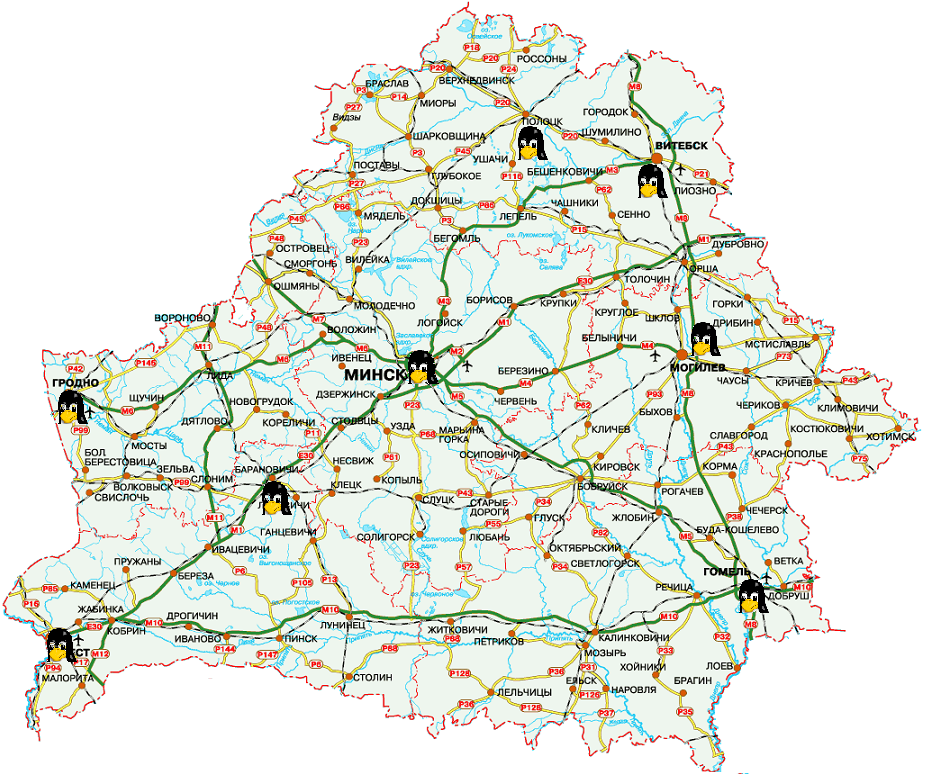
\includegraphics[width=7cm]{03_2012_bilorus}
  \label{fig:Zlobin1}
  \caption{Выкарыстанне СПЗ у ВНУ Беларусі}
\end{figure}


\subsection*{Выкарыстанне СПЗ ў ВНУ Расійскай Федэрацыі}

У адрозненні ад Беларусі ў Расійскай Федэрацыі ў 2008 г. была прынята канцэпцыя
развіцця распрацоўкі і выкарыстання свабоднага праграмнага забеспячэння. У
рамках гэтай канцэпцыі ў 2008-2010 гг. была рэалізавана праграма выкарыстання
СПЗ у школах Расійскай Федэрацыі (у 35\% школ СПЗ устаноўлена больш чым на
50\% кампутараў). Трэба адзначыць, што ў адрозненне ад Беларусі і Украіны ў
Расійскай Федэрацыі назіраецца некаторая актыўнасць кантралюючых органаў з
нагоды ліцэнзійнага праграмнага забеспячэння. Самай рэзананснай справай была
справа А.М. Понасава, якая і прывяла да стварэння ў 2008 г. грамадскай арганізацыі
<<Цэнтр вольных тэхналогій>>. Як вынікае з  \cite{Zlobin1, Zlobin2, Zlobin3}, у большасці ВНУ
Расійскай Федэрацыі назіраецца выкарыстанне як Microsft Windows, так і GNU/Linux. Толькі
ў некаторых ВНУ кіраўніцтвам прынята валявое рашэнне аб поўным пераходзе на
СПЗ (Санкт-Пецярбургскі гандлёва-эканамічны універсітэт, Томскі дзяржаўны
педагагічны універсітэт, Ніжагародскі радыётэхнічны каледж). Як і ў Беларусі
выкарыстанне СПЗ у ВНУ Расійскай Федэрацыі можна падзяліць на тры напрамкі
\cite{Zlobin3, Zlobin4, Zlobin5}:

\begin{enumerate}
  \item \textbf{праграмнае забеспячэнне падтрымкі навучальнага \linebreak працэсу} (у асноўным
  сістэмнае праграмнае забеспячэнне на серверах і працоўных станцыях). У
  большасці выпадкаў сістэмнае СПЗ на працоўных станцыях прадстаўлена GNU/Linux
  у рэжыме мультызагрузкі як альтэрнатыўная АС у кампутарных класах кафедраў;
  \item \textbf{дадатковае праграмнае забеспячэнне, якое выкарыстоўваецца студэнтамі
  пры самастойнай працы} (на \linebreak жаль аўтары не валодаюць дадзенымі аб гэтай групе
  СПЗ);
  \item \textbf{праграмнае забеспячэнне для выкарыстання ў навучальных курсах.}
  У гэтым кірунку спектр СПЗ значна шырэй, чым у Беларусі. Тут можна згадаць
  выкарыстанне СПЗ для вывучэння праграмавання на мовах С/C++ (у Яраслаў\-скім
  Універсітэце ёсць цікавы вопыт навучання праграмаванню на аснове СПЗ), Pascal
  (Free Pascal, Lazarus), Java, Haskel, Prolog; SciLab, Octave, Sage для выканання матэматычных разлікаў
  (шырокі вопыт выкарыстання вольнага матэматычнага праграмнага забеспячэння
  назапашаны ва універсітэтах Новасібірска, Барнаула, Бійска); арганізацыя
  сістэм дыстанцыйнага навучання, выкарыстанне свабодных сістэм віртуалізацыі
  для вывучэння аперацыйных сістэм; інструментар для філалагічнага аналізу
  тэкстаў; выкарыстанне інструментара верыфікацыі ПЗ у падрыхтоўцы магістраў;
  стварэнне электронных адукацыйных рэсурсаў падтрымкі навучальнага працэсу
  для завочнай формы навучання (аўтары разумеюць, што рэальны спіс выкарыстанага
  СПЗ значна шырэй, але ў адкрытым доступе дадзеных пакуль што няма).
\end{enumerate}

У ВНУ Расійскай Федэрацыі даволі актыўна выкарыстоўваюцца вылічальныя
кластары з выкарыстаннем СПЗ. Па ініцыятыве рэктараў МДУ ім. М.В. Ламаносава,
Ніжагародскага універсітэта ім. М.І. Лабачэўскага, Томскага дзяржаўнага
універсітэта, Паўднёва-Уральскага дзяржаўнага універсітэта створаны
<<Суперкампутарны кансорцыум універсітэтаў Расіі>>. У спіс TOP500 ад снежня 2011
г. уваходзяць чатыры расейскія суперкампутара (\No 18, 107, 119, 121).

Варта адзначыць, што ў Расійскай Федэрацыі назапашаны значны вопыт
распрацоўкі свабоднага праграмнага забеспячэння. У Расеі распрацоўваюцца
дыстрыбутывы GNU/Linux: ALT Linux (\url{http://altlinux.ru}), Calculate Linux (\url{http://www.calculate-linux.ru}), ROSA
(\url{http://rosalab.ru}). Наяўнасць кампаній, якія займаюцца распрацоўкай СПЗ, дазваляе
распрацоўваць спецыялізаваныя свабодныя праграмы і значна спрашчае рэалізацыю
праектаў па ўкараненні GNU/Linux у школы і універсітэты.

\begin{figure}[htpb]
  \centering
  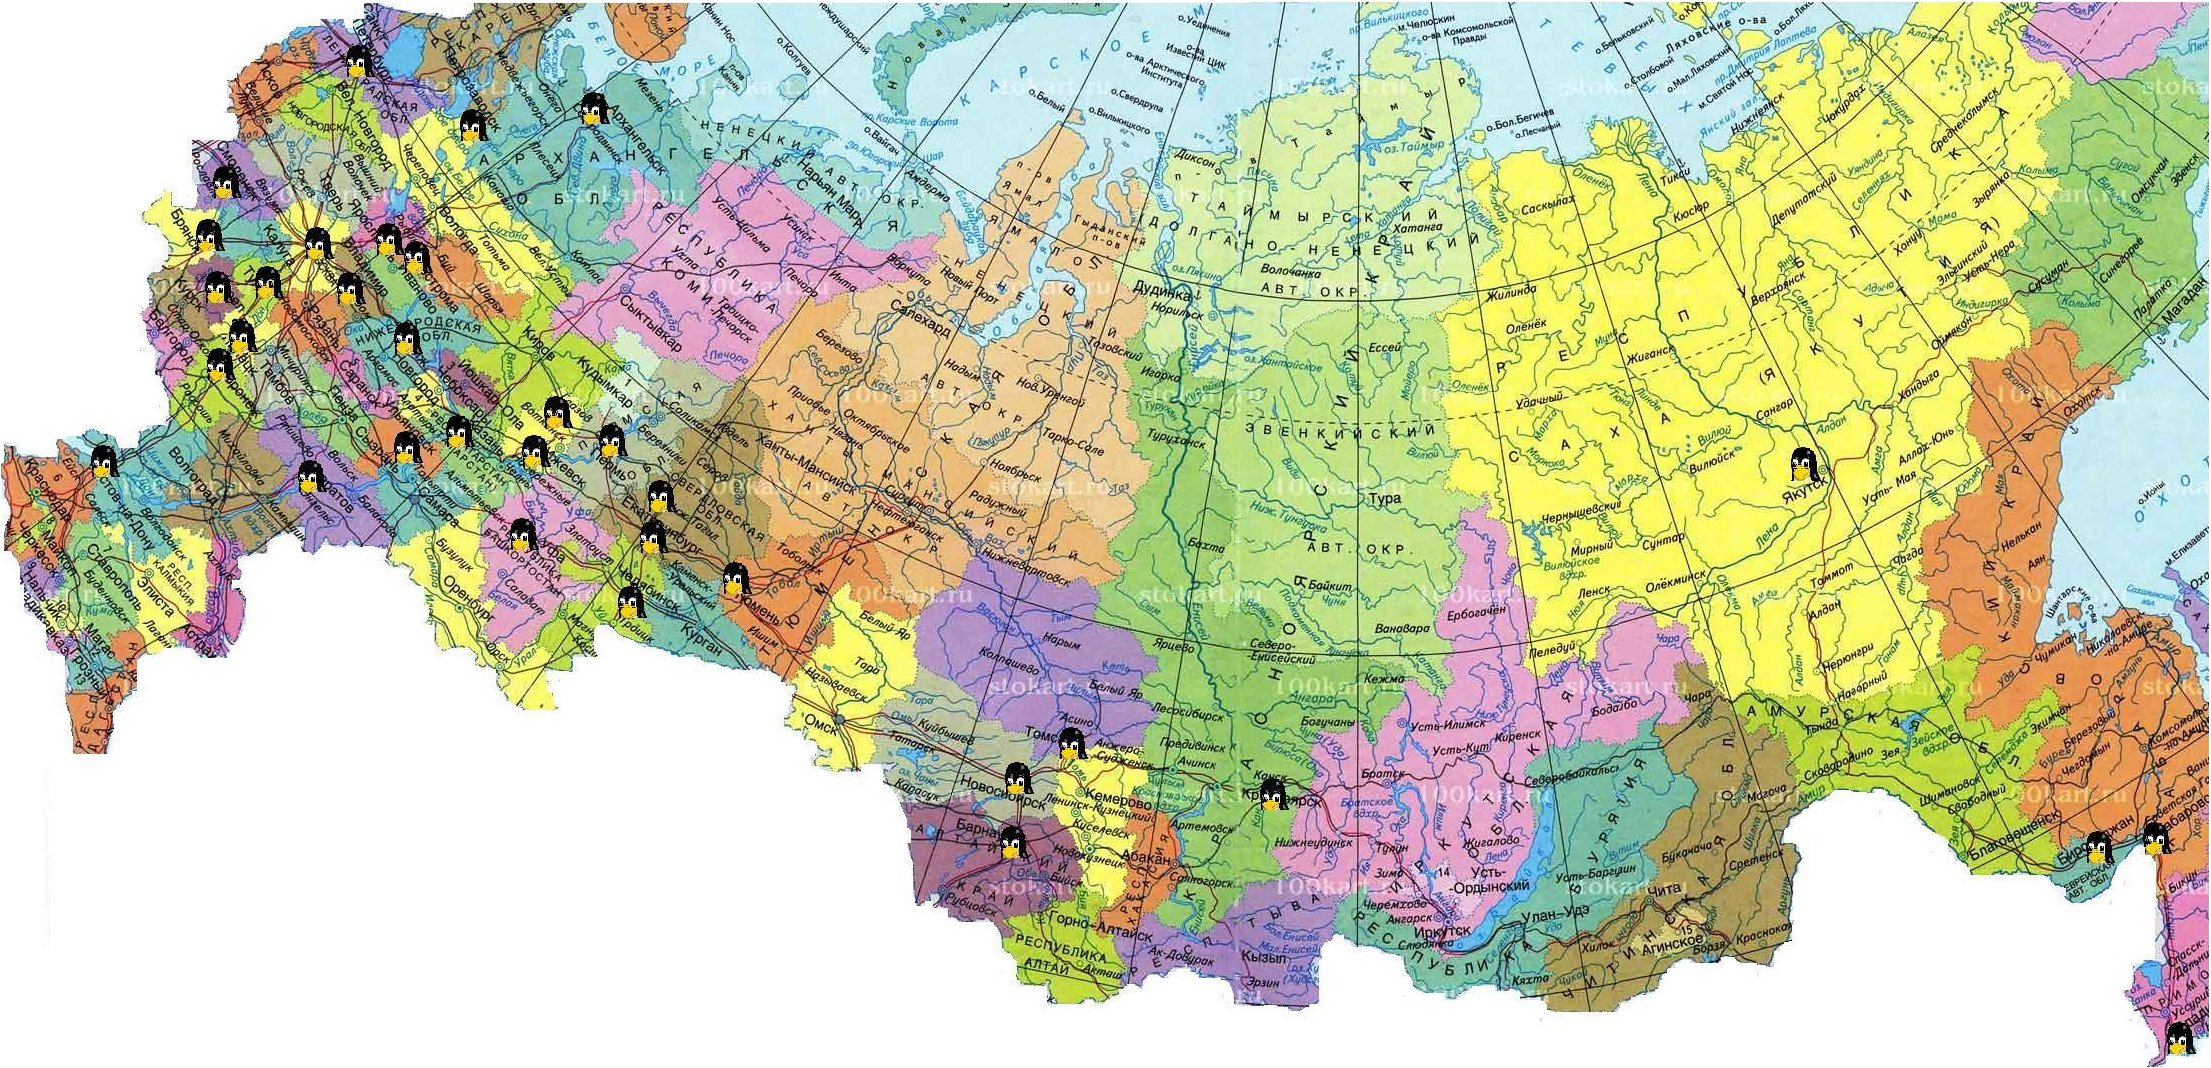
\includegraphics[width=11cm]{03_2012_russia2_with_tux}
  \label{fig:Zlobin2}
  \caption{Выкарыстанне СПЗ у ВНУ Расійскай Федэрацыі}
\end{figure}

\subsection*{Выкарыстанне СПЗ у ВНУ Украіны}

Ва Украіне <<Дзяржаўная мэтавая навукова-тэхнічная праграма выкарыстання ў
органах улады праграмнага забеспячэння з адкрытым кодам>> была зацверджана
ў 2010 г., але да рэальнага яе выканання пакуль што не дайшлі. У адрозненне ад
Расійскай Федэрацыі праверкі адпаведнымі дзяржаўнымі органамі выпадкаў
парушэння аўтарскіх правоў уласнікаў праграм праводзяцца ў значна меншым аб'ёме
і пераважна ў гасразліковых арганізацыях. Вядомыя толькі асобныя выпадкі такіх
праверак у ВНУ. Як і ў Беларусі пакуль што адсутнічае эканамічны складнік
у выбары праграмнага забеспячэння для ВНУ. Пасля набыцця ПЭВМ пераважна
з ліцэнзійнымі Microsoft Windows і Microsoft Office устанаўліваецца вялікая колькасць
неліцэнзійнага ПЗ, чым зводзяцца дарэмна фантастычна вялікія выдаткі сродкаў
на першаснае набыццё ПА (Львоўскі нацыянальны універсітэт імя Івана Франка
да эканамічнага крызісу 2008 г. кожны год купляў прыблізна 1000 ПЭВМ. Сумарній
кошт ліцэнзій толькі на Microsoft Windows (ОЭМ-версія) і Microsoft Office складал амаль 300000
у.а. на год--даволі вялікая сума, як для ЛНУ ім.і.Франка!). У большасці выпадкаў
выбар менавіта прапрыетарнага ПЗ звязаны нават не са спажывецкімі якасцямі
гэтых праграм, а фактам павярхоўнага знаёмства выкладчыка з гэтай праграмай
ці нават наяўнасцю ў яго якой-небудзь кніжкі з апісаннем праграмы. Разам з
тым, выступленні выкладчыкаў і навуковых супрацоўнікаў на першай і другой
канферэнцыі FOSS Lviv  \cite{Zlobin1, Zlobin2} сведчаць аб шырокім спектры выкарыстання СПЗ
у ВНУ Украіны.

Як і ў Беларусі і Расійскай Федэрацыі выкарыстанне СПЗ у ВНУ Украіны можна
падзяліць на тры напрамкі \cite{Zlobin1, Zlobin2}:

\begin{enumerate}
  \item \textbf{праграмнае забеспячэнне падтрымкі навучальнага \linebreak працэсу (у асноўным
  сістэмнае праграмнае забеспячэнне на серверах і працоўных станцыях).} У
  большасці выпадкаў сістэмнае СПЗ на працоўных станцыях прадстаўлена GNU/Linux
  у рэжыме мультызагрузкі, як альтэрнатыўная АС у кампутарных класах кафедраў;
  \item \textbf{дадатковае праграмнае забеспячэнне, якое выкарыстоўваецца студэнтамі
  падчас іх самастойнай працы} (на жаль, аўтары на сённяшні дзень не маюць
  дадзеных аб гэтай групе СПЗ);
  \item \textbf{праграмнае забеспячэнне для выкарыстання ў навучальных курсах.}
  У гэтым кірунку спектр СПЗ значна шырэй, чым у Беларусі. Гэта выкарыстанне
  сістэм кампутарнай матэматыкі; арганізацыя сістэм дыстанцыйнага навучання,
  выкарыстанне свабодных сістэм віртуалізацыі для вывучэння аперацыйных сістэм;
  выкарыстанне СПЗ для тэставання апаратнага забеспячэння ПЭВМ; выкарыстанне
  офіснага пакета OpenOffice.org.ukr у курсе інфарматыкі ВНУ; выкарыстанне адкрытых
  сродкаў праграмавання ў навучанні і ў навуковых даследаваннях; (аўтары аддаюць
  сабе справаздачу ў тым, што рэальны спіс прымяняемага СПЗ значна шырэй, але
  больш поўныя дадзеныя аб гэтым аўтарам невядомыя).
\end{enumerate}

У ВНУ Украіны эксплуатуюцца вылічальныя кластары с выкарыстаннем СПЗ, нараўне
са спецыялізаванымі ўстаноўкамі шырока выкарыстоўваюцца размеркаваныя
кластарныя сістэмы і сістэмы з выкананнем вылічэнняў на графічных працэсарах.

У выніку можна канстатаваць як шырокі спектр выкарыстання СПЗ ва ўкраінскіх
ВНУ ад дыстанцыйнага навучання да распрацоўкі СПЗ, так і шырокую геаграфію
выкарыстання СПЗ ад Луганска на ўсходзе да Львова на захадзе і ад Чарнігава
на поўначы да Адэсы на поўдні.

\begin{figure}[htpb]
  \centering
  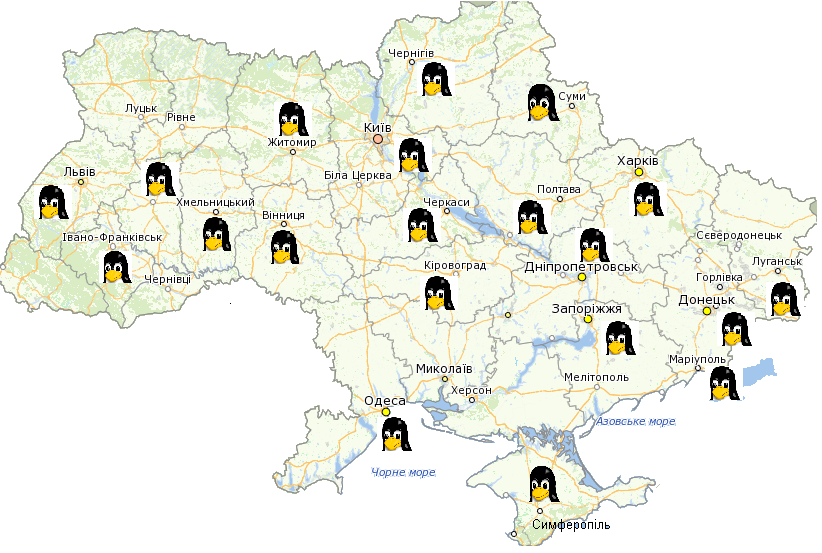
\includegraphics[width=07cm]{03_2012_ukraine}
  \label{fig:Zlobin3}
  \caption{Выкарыстанне СПЗ у ВНУ Украіны}
\end{figure}

Падводзячы вынікі, можна канстатаваць, што:

\begin{enumerate}
  \item незалежна ад наяўнасці або адсутнасці канцэпцыі выкарыстання СПЗ, яно
  выкарыстоўваецца ў ВНУ Беларусі, Расійскай Федэрацыі і Украіны;
  \item колькасна аб'ём выкарыстання СПЗ у адукацыі вышэй у Расійскай Федэрацыі;
  \item ва ўсіх трох краінах міністэрства адукацыі займаюць адхіленую пазіцыю ў
  працэсе ўкаранення СПЗ ва універсітэты і школы;
  \item ва ўсіх трох краінах узровень выкарыстання СПЗ у ВНУ з'яў\-ляец\-ца
  недастатковым. Свабода выбару ПЗ, якой карыстаюцца выкладчыкі ВНУ, у большасці
  выпадкаў не прыводзіць да выбару найлепшага інструментара, а абумоўлена
  звычкамі альбо стэрэатыпамі (часта памылковымі) выкладчыкаў.
\end{enumerate}

\begin{thebibliography}{9}

\bibitem{Zlobin1} Тези доповідей міжнародної науково-практичної конференції FOSS Lviv-2011. ---
Львів.: Львівський національний університет імені Івана Франка, 2011. --- 196 с.

\bibitem{Zlobin2} Друга міжнародна науково-практична конференція FOSS Lviv-2012: Збірник
наукових праць/ Львів, 26-28 квітня 2012 р. --- 160 с.

\bibitem{Zlobin3} Алексеев Е.Р., Брагилевский В.Н. Использование свободного програмного
обеспечения в университетах и исследовательских учреждений Российской
Федерации. Друга міжнародна науково-практична конференція FOSS Lviv-2012: Збірник
наукових праць/ Львів, 26-28 квітня 2012 р.

\bibitem{Zlobin4} В.Н. Брагилевский, С.А. Гуда, Г.В. Худолей СПО на мехмате Южного
федерального университета. Седьмая конференция <<Свободное программное
обеспечение в высшей школе>>: Тезисы докладов/ Переславль, 28-29 января 2012 года. М.:
Альт Линукс, 2012. 110 с.: ил.

\bibitem{Zlobin5} \url{lists.raspo.ru/Plone/publichnye-drafty-dokumentov/dokumenty-komiteta-po-obrazovaniyu-i-vysshei-shkole/spo-v-rossiiskih-vuzah}

\bibitem{Zlobin6} Derechennik S.S., Kostiuk D.A., Pynkin D.A. Free/libre software usage in the belarusian system of higher educational
institutions // Друга міжнародна науково-практична конференція FOSS Lviv-2012: Збірник
наукових праць/ Львів, 26-28 квітня 2012 р.

\end{thebibliography}

\end{document}




